% Data sythesis using the Robinson/Freyer/Hindriks model - Model Description
% Written by Christopher Thomas.

\chapter{Robinson Model}
\label{sect-robinson}

\fixme{Edit this.}

The model presented in Robinson 2002 (hereafter ``the Robinson model'')
provides a series of differential equations relating the firing rates of
multiple neural populations in the cortex and thalamus. Feedback between
these regions drives noise-excited oscillations.

The most relevant references are:
\begin{itemize}
\item Robinson 2002 -- Describes the model, finds steady-state points, and
analyzes perturbations around those points to find oscillation modes.
\item Freyer 2011 -- Describes an extension to the model where noise is
modulated by the network's own output, providing a closer match to the
distribution of oscillation modes in biological data.
\item Hindriks 2023 -- Describes an extension to the model that adds multiple
independent copies of the Robinson and Freyer model, with coupling between
instances. This is used to model co-oscillation of different brain regions
in biological data.
\end{itemize}
(See Section \ref{sect-robinson-refs} for citations.)

%
%
\section{Model Description}
\label{sect-robinson-model}

A diagram of the Robinson model with the extensions from Freyer 2011 and
Hindriks 2023 is shown in Figure \ref{fig-robinson-diagram}. To distinguish
this from the Robinson 2002 model, this will be referred to as ``the
extended Robinson model''.

\figdef{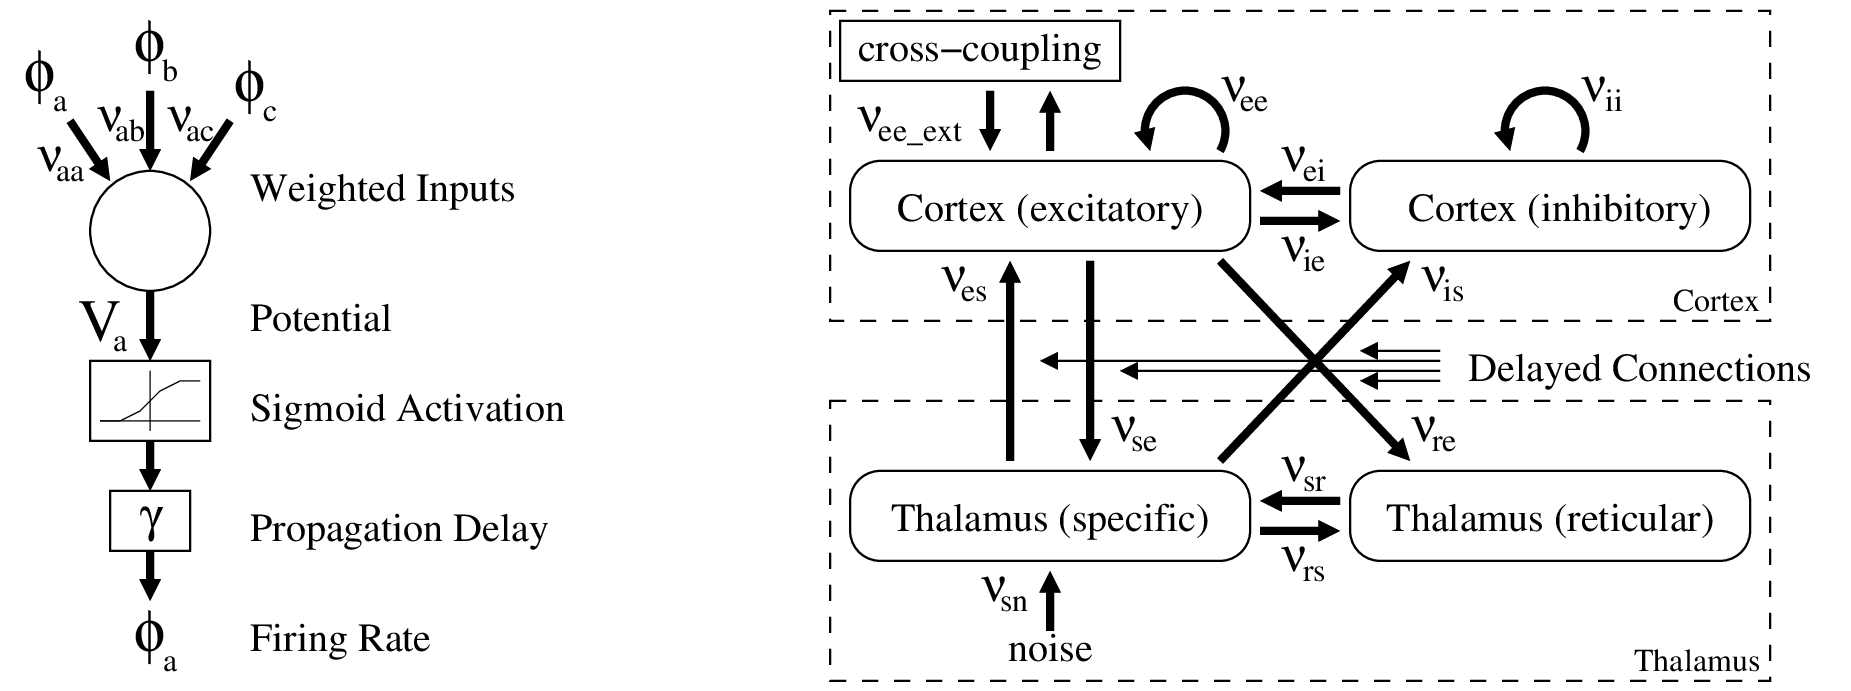
\includegraphics[width=0.9\columnwidth]{figures/robinson-model}}
{Extended Robinson model diagram, showing the neuron population model
(left) and the population interactions (right).}{fig-robinson-diagram}

The neural population model is described in Equations
\ref{eq-robinson-potential}, \ref{eq-robinson-sigmoid} and
\ref{eq-robinson-gamma}.
%
Per Equation \ref{eq-robinson-potential}, a weighted sum of input firing
rates $\phi_b(t)$ is used to generate the cell body potential $V_a(t)$. A
single dot indicates the first time derivative, and a double dot indicates
the second time derivative. The parameters $\alpha$ and $\beta$ are the
inverse of the membrane potential fall time and rise time, respectively.
The coupling parameter $\nu_{ab}$ is the strength of the connection from
region $b$ to region $a$ (zero if no connection, negative if inhibitory).

\textbf{NOTE:} A delay is manually applied to some of the $\phi_b$ signals
before this summation to reflect signal propagation time between the cortex
and thalamus (per Robinson 2002), and to reflect cross-coupling delays
within the cortex populations (per Hindriks 2023).

\begin{equation}
\left ( \frac{1}{\alpha \beta} \right ) \ddot{V}_a(t)
+ \left ( \frac{1}{\alpha} + \frac{1}{\beta} \right ) \dot{V}_a(t)
+ V_a(t) = \sum_b \nu_{ab} \phi_b(t)
\label{eq-robinson-potential}
\end{equation}

Per Equation \ref{eq-robinson-sigmoid}, the cell body potential $V$ is fed
into a sigmoid activation function, to represent the collective action of
many neurons with varying firing thresholds. The mean firing threshold is
$V_{th}$ and the standard deviation of the threshold is $\sigma_{th}$.
This follows the convention of Freyer 2011; Robinson 2002 defined a
related parameter $\sigma'_{th} = \frac{\sqrt{3}}{\pi} \sigma_{th}$ to
simplify the activation equation (Equation \ref{eq-robinson-sigmoid-prime}).

\begin{equation}
Q(V) = \frac{Q_{max}}
{1 + e^{- \left ( \frac{\pi}{\sqrt{3}} \right )
\left ( \frac{ V - V_{th}}{\sigma_{th}} \right )}}
\label{eq-robinson-sigmoid}
\end{equation}

\begin{equation}
Q(V) = \frac{Q_{max}}
{1 + e^{- \left ( \frac{ V - V_{th}}{\sigma'_{th}} \right )}}
\label{eq-robinson-sigmoid-prime}
\end{equation}

Per Equation \ref{eq-robinson-gamma}, the local firing rate $Q$ is
propagated with damping and finite delay to give the non-local firing rate
$\phi$. A single dot indicates the first time derivative, and a double dot
indicates the second time derivative. Per Robinson 2002, local propagation
delay is assumed to only be relevant within the cortex, and
$\gamma = \infty$ is assumed elsewhere. Per Freyer 2011, this further only
applies to the excitatory neuron populations in the cortex.

\begin{equation}
\left \{
\begin{array}{rcl}
\frac{1}{\gamma^2} \ddot{\phi}(t) + \frac{2}{\gamma} \dot{\phi}(t) + \phi(t)
= Q(t) & ~~ & \mathrm{Cortex ~ excitatory ~ neurons.} \\
\phi(t) = Q(t) & ~~ & \mathrm{All ~ other ~ populations.} \\
\end{array}
\right .
\label{eq-robinson-gamma}
\end{equation}

Noise is injected into the model as $\phi_n$, and is described by Equation
\ref{eq-robinson-noise}. Per Freyer 2011, there are three components:
constant, additive, and multiplicative. Multiplicative noise (noise
modulated by $\phi_e$) is important for broadening the distribution of
peak power levels of transient oscillations at frequencies above the
fundamental oscillation mode of the cortex/thalamus loop.

In Equation \ref{eq-robinson-noise}, $\phi_n$ is the noise coupled to
the thalamus via $\nu_{sn}$, $\mu_n$ is the constant noise component
(background firing rate), $\sigma_n$ is the standard deviation of the
independent component of the noise, and $\chi$ is a scaling parameter
(per Freyer 2011) such that $\sigma_n \chi$ is the standard deviation of
the component of the noise that is modulated by $\phi_e$. Since the $\phi_e$
signal has to propagate from the cortex to the thalamus before modulating
this noise component, it is manually delayed. The signals $g_1(t)$ and
$g_2(t)$ denote two independent Gaussian noise sources with zero mean and
with standard deviations of 1.

\begin{equation}
\phi_n(t) = \mu_n + \sigma_n g_1(t)
+ \sigma_n \chi g_2(t) \phi_e(t - t_{halfloop})
\label{eq-robinson-noise}
\end{equation}

As shown in Figure \ref{fig-robinson-diagram}, cross-coupling between
excitatory cortical populations is implemented per Hindriks 2023. This is
described by Equation \ref{eq-robinson-coupling}. Weight values
$w_{ab}$ represent the strength of connections between populations, and
delay values $t_{coupling_{ab}}$ represent the propagation delays of these
connections.
While arbitrary weight values may be chosen, the recommended implementation
is to use positive weights (purely excitatory), with the constraint that the
sum of all weights contributing to a given $\phi_{ext_k}$ should sum to
approximately unity. Cross-coupling propagation delay is typically no more
than $\frac{1}{\gamma}$.

\begin{equation}
\phi_{ext_a}(t) = \sum_b w_{ab} \phi_{e_b}(t - t_{coupling_{ab}})
\label{eq-robinson-coupling}
\end{equation}
%
\begin{equation}
\forall a, \sum_b w_{ab} \approx 1
\label{eq-robinson-coupling-constraint}
\end{equation}

Typical parameter values for the extended Robinson model are shown in
Table \ref{tab-robinson-params}. Typical coupling coefficients are shown in
Table \ref{tab-robinson-couplings}. These are very similar to the parameter
and coupling coefficient values used in Hindriks 2023.

\tabdef{%
\begin{tabular}{cccl}\hline
\textbf{Parameter} & \textbf{Value} & \textbf{Units} & \textbf{Notes} \\
\hline
$Q_{max}$ & 250 & sec$^{-1}$ & maximum firing rate \\
$V_{th}$ & 15 & mV & potential threshold for firing \\
$\sigma_{th}$ & 6 & mV & standard deviation of firing threshold \\
\hline
$\alpha$ & 50 & sec$^{-1}$ & membrane potential inverse fall time \\
$\beta$ & 200 & sec$^{-1}$ & membrane potential inverse rise time \\
$\gamma$ & 100 & sec$^{-1}$ & cortex inverse propagation delay \\
\hline
$t_{halfloop}$ & 40 & ms & one-way cortex/thalamus delay \\
\hline
$\mu_n$ & 0 & sec$^{-1}$ & constant noise firing rate \\
$\sigma_n$ & 0.1 & sec$^{-1}$ & additive noise standard deviation \\
$\chi$ & 0.3 & dimensionless & multiplicative noise deviation coefficient \\
\hline
\end{tabular}
}{Typical parameters for the extended Robinson model.}
{tab-robinson-params}

\tabdef{%
\begin{tabular}{cc}
\hline
$\nu_{ee}$ & 1.2 \\
$\nu_{ei}$ & -1.8 \\
$\nu_{es}$ & 1.2 \\
\hline
$\nu_{ie}$ & 1.2 \\
$\nu_{ii}$ & -1.8 \\
$\nu_{is}$ & 1.2 \\
\hline
$\nu_{se}$ & 1.2 \\
$\nu_{re}$ & 0.4 \\
\hline
$\nu_{sr}$ & -0.8 \\
$\nu_{rs}$ & 0.2 \\
\hline
$\nu_{sn}$ & 0.5 \\
\hline
$\nu_{ee_{ext}}$ & 0.07 \\
\hline
\end{tabular}
}{Typical coupling coefficient values for the extended Robinson model.}
{tab-robinson-couplings}

Robinson 2002 describes several oscillating modes: slow-wave/delta-wave
oscillation, theta/fast~delta oscillation with stable frequency (3~Hz) but
varying shape, spindle oscillations at about 10~Hz driven by intra-thalamic
resonance, and alpha oscillations at about 10~Hz. These are parameterized
in terms of the amplification provided by each population of neurons
(Equations 13-15 and Figure 3 in that reference).

The parameter values used in Freyer 2011 and Hindriks 2023 were chosen to
support biologically relevant oscillations when driven by external noise.

%
%
\section{References}
\label{sect-robinson-refs}

\begin{itemize}
%
\item P. A. Robinson, C. J. Rennie, and D. L. Rowe, \textit{Dynamics of
Large-Scale Brain Activity in Normal Arousal States and Epileptic Seizures},
Physical Review E, 65, 041924, April 2002
%
\item F. Freyer, J. A. Roberts, R. Becker, P. A. Robinson, P. Ritter, and
M. Breakspear, \textit{Biophysical Mechanisms of Multistability in
Resting-State Cortical Rhythms}, Journal of Neuroscience, 31,
pp 6353--6361, April 2011
%
\item R. Hindriks and P. K. B. Tewarie, \textit{Dissociation Between Phase
and Power Correlation Networks in the Human Brain is Driven by Co-Occurrent
Bursts}, Communications Biology, 6, 286, March 2023
%
\end{itemize}

%
%
% This is the end of the file.
